\documentclass{beamer}
%\documentclass[handout]{beamer}
\usetheme{Darmstadt}

\usepackage[utf8]{inputenc}
\usepackage{default}
\usepackage{hyperref}
\hypersetup{colorlinks=true,urlcolor=orange}
\usepackage{tikz}
\usepackage{lipsum} % <= to insert dummy text
\usepackage[absolute,overlay]{textpos}

\newcommand{\tango}{\textsc{Tango}}
\newcommand{\corba}{\textsc{Corba}}
\newcommand{\onmiORB}{\textsc{omniORB}}
\newcommand{\zmq}{\textsc{$\varnothing$mq}}
\newcommand{\mysql}{\textsc{MySQL}}
\newcommand{\sardana}{\textsc{Sardana}}
\newcommand{\mambo}{\textsc{Mambo}}
\newcommand{\atk}{\textsc{Atk}}
\newcommand{\taurus}{\textsc{Taurus}}
\newcommand{\spock}{\textsc{Spock}}

\newcommand{\todo}[1]{\texttt{\color{red}TODO:} ``\emph{#1}''}

\newcommand{\Fp}{\ensuremath{\mathbb{F}_p}}%                    Cuerpo finito de orden p (primo)

\title[Securing \tango\, Control System]{Securing \tango\, Control System:\\ A brainstorming}
\author[Sergi Blanch-Torn\'e]{Sergi Blanch i Torn\'e}
\institute[Universidad de Lleida]{Cryptography \& Graphs\\Math Department\\ Universitat de Lleida}
\date{September 24th, 2013}

\begin{document}

%------------------------------------ Frame 0.1 ------------------------------%
%\frame{\titlepage}
\begin{frame}
    \titlepage
    \begin{textblock*}{10mm}(0.55\textwidth,0.95\textheight)
         \href{http://creativecommons.org/licenses/by-nc-sa/3.0/deed.es_CO}{
             
\includegraphics[width=\textwidth]{imgs/aux/by-nc-sa_eu_petit.png}
         }
    \end{textblock*}
\end{frame}
%-----------------------------------------------------------------------------%

%------------------------------------ Frame 0.2 ------------------------------%
\begin{frame}
\frametitle{Outline}
\tableofcontents[hideallsubsections]
\end{frame}
%-----------------------------------------------------------------------------%

%%%%%%%%%%%%%%%%%%%%%%%%%%%%%%%%%%%%%%%%%%%%%%%%%%%%%%%%%%%%%%%%%%%%%%%%%%%%%%%
\section{Introduction}

\subsection{Definitions}

%------------------------------------ Frame 1.1 ------------------------------%
\begin{frame}
\frametitle{What is an Industrial Control System? (ICS)}
    \begin{block}{\href{http://en.wikipedia.org/wiki/Industrial_Control_System}{Wikipedia's definition (en)}}
        ``It is a general term that encompasses several types of control systems used in industrial production, including \emph{supervisory control and data acquisition} (\alert<3->{SCADA}) systems, \emph{distributed control systems} (\alert<4->{DCS}), and other smaller control system configurations such as \emph{programmable logic controllers} (\alert<2->{PLC}) often found in the industrial sectors and critical infrastructures.''
    \end{block}
\end{frame}
%-----------------------------------------------------------------------------%

%------------------------------------ Frame 1.2 ------------------------------%
\begin{frame}
    \begin{exampleblock}{What is a Programmable Logic Controllers?}
        \begin{figure}
            \centering{
                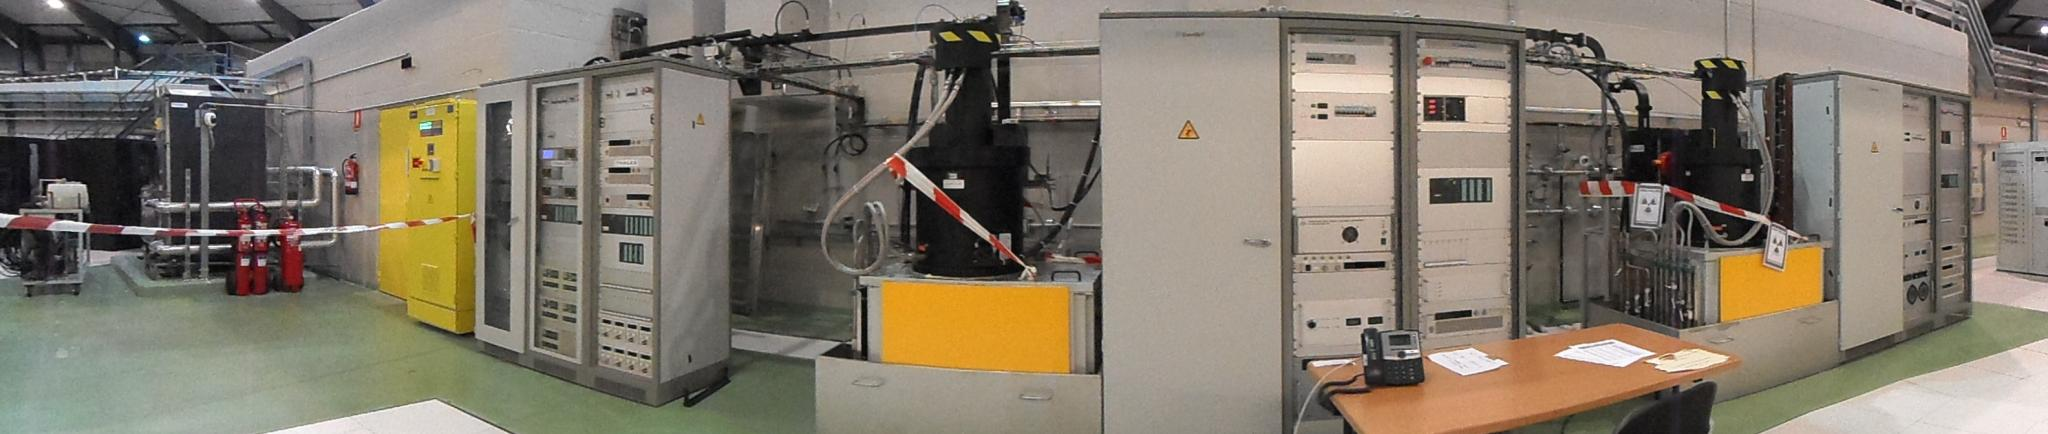
\includegraphics[width=0.9\textwidth]{imgs/alba/20130812_101456_015.jpg}
            }
        \end{figure}
        \begin{figure}
            \centering{
                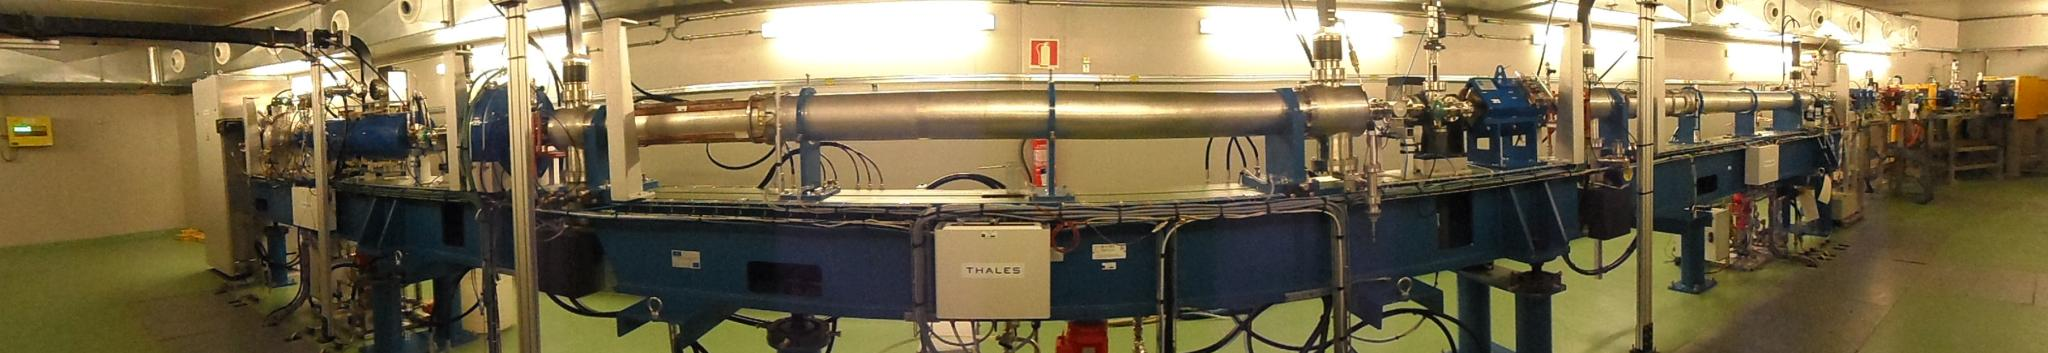
\includegraphics[width=0.9\textwidth]{imgs/alba/20130812_101743_023.jpg}
                \caption{Example of a PLC controlled system}\label{fig:linacPLCs}
            }
        \end{figure}
    \end{exampleblock}
    \begin{textblock*}{60mm}(0.25\textwidth,0.5\textheight)
        \begin{exampleblock}{}<2->
            This a production line like example!
        \end{exampleblock}
    \end{textblock*}
\end{frame}
%-----------------------------------------------------------------------------%

%------------------------------------ Frame 1.3 ------------------------------%
\begin{frame}
\frametitle{What is an SCADA?}
    \begin{block}{\href{http://es.wikipedia.org/wiki/SCADA}{Wikipedia's definition (es)}}
        ``\emph{Supervisory Control And Data Acquisition} it is a computer software to control and supervise industrial process remotely.''
    \end{block}
    \begin{exampleblock}{Examples of an SCADAs}<2->
        \begin{figure}[h]
            \centering{
            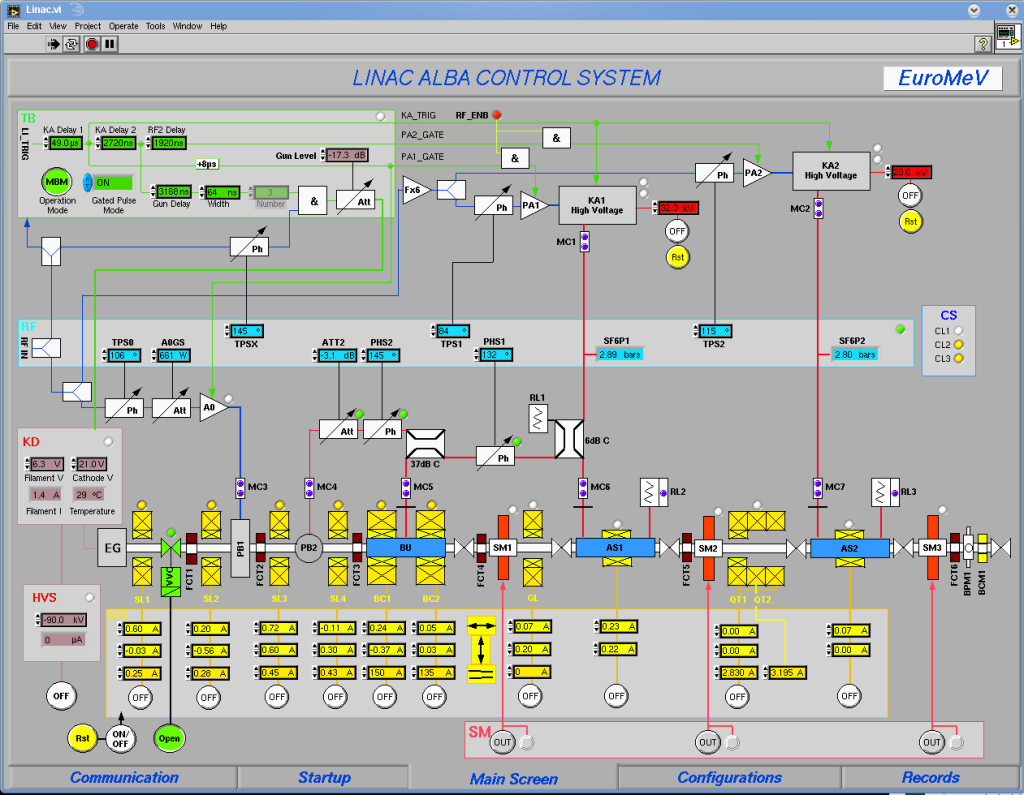
\includegraphics[width=0.4\textwidth]{imgs/alba/labview_tab3_mainScreen.png}
            \caption{Labview as SCADA example} \label{fig:labviewScada}}
        \end{figure}
    \end{exampleblock}
\end{frame}
%-----------------------------------------------------------------------------%

%------------------------------------ Frame 1.4 ------------------------------%
\begin{frame}
\frametitle{What is an Distributed Control System?}
    \begin{block}{\href{http://en.wikipedia.org/wiki/Distributed_control_system}{Wikipedia's definition (en)}}
        a \emph{Distributed Control System} is the computer software for a manufacturing system, process or any kind of dynamic system, in which the controller elements are not central in location (like the brain) but are distributed throughout the system with each component sub-system controlled by one or more controllers.
    \end{block}
    \begin{block}{What is a distributed system?}
        Tanenbaum say \cite{TanenbaumDistr}: \emph{A distributed system is a collection of independent computers that appears to its users as a single coherent system.}
    \end{block}
\end{frame}
%-----------------------------------------------------------------------------%

%------------------------------------ Frame 1.5 ------------------------------%
\begin{frame}
\frametitle{What is a \tango? (I)}
    \tango is an object oriented \emph{Distributed Control System}\\with active collaborative development from:
    \begin{figure}[h]
        \centering{
        
\includegraphics[width=0.45\textwidth]{imgs/tango/00_logos_tango_consortium_members.jpg}
        \caption{Logos of the Tango Consortium Members} \label{fig:tangoConsortium}}
    \end{figure}
    Together with tools like \sardana, \taurus, \atk\, and \mambo\, there is a big \emph{Industrial Control System}\\
    Them can act as an SCADA and/or DCS flexibly to the needs.
\end{frame}
%-----------------------------------------------------------------------------%

%------------------------------------ Frame 1.6 ------------------------------%
\begin{frame}
\frametitle{What is a \tango? (II)}
    \begin{block}{It's an Distributed Control System}
        using \corba\, as a Middleware (\onmiORB),\\ with \zmq\, in the event broadcasting.
    \end{block}
    \begin{block}{What means middleware?}
        Tanenbaum say \cite{TanenbaumDistr}: \emph{It is what supports heterogeneous computers and networks while offering a single system view.}
    \end{block}
\end{frame}
%-----------------------------------------------------------------------------%

%------------------------------------ Frame 1.7 ------------------------------%
\begin{frame}
\frametitle{What is a \tango? (\&III)}
    \begin{block}{\tango\, parts}
        \begin{itemize}
            \item \tango\, core $\Rightarrow$ the Middleware
            \item \tango\, Device Servers $\Rightarrow$ the agents in the DCS
        \end{itemize}
    \end{block}
    \begin{exampleblock}{Device servers, device classes, and devices}
        \begin{figure}[h]
            \centering{
                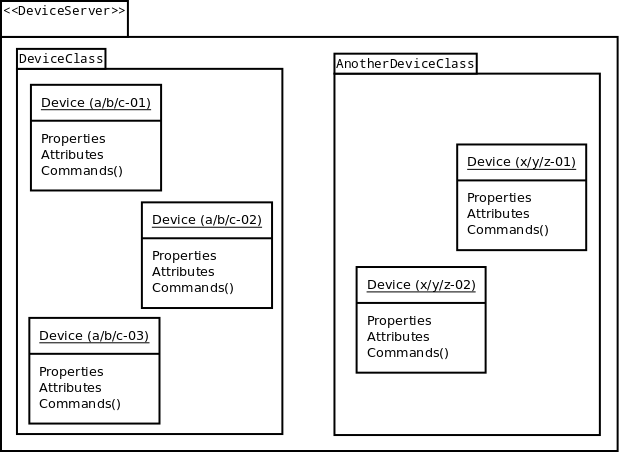
\includegraphics[width=0.7\textwidth]{imgs/tango/tango_DeviceServer_DeviceClass_Device.png}
            }
        \end{figure}
    \end{exampleblock}
\end{frame}
%-----------------------------------------------------------------------------%

%------------------------------------ Frame 1.8 ------------------------------%
\begin{frame}
    \begin{figure}[h]
        \centering{
            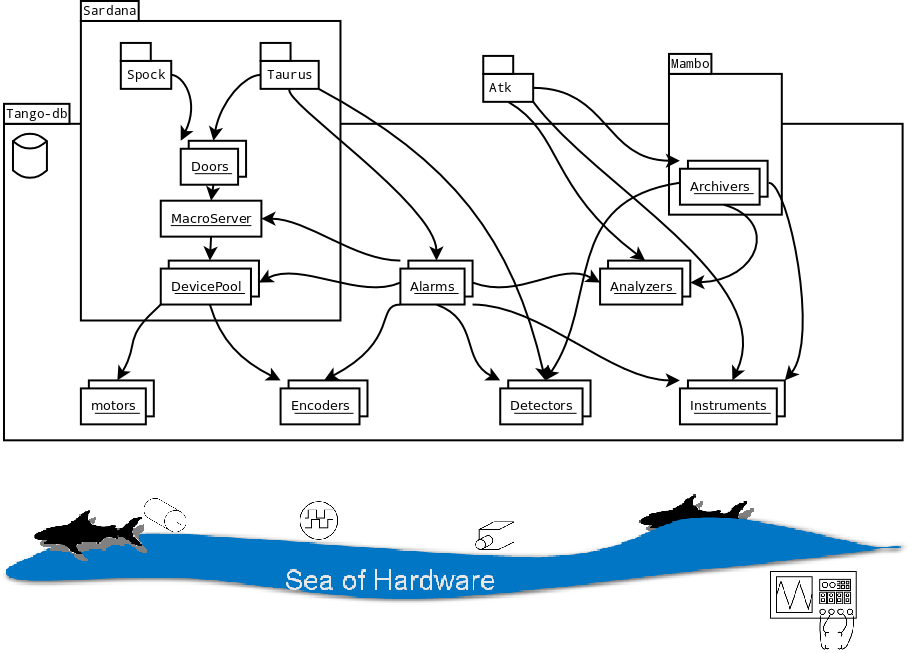
\includegraphics[width=0.75\textwidth]{imgs/tango/tango_layout.png}
            \caption{Tango schematic layout} \label{fig:tangoLayout}
        }
    \end{figure}
    \begin{textblock*}{60mm}(0.05\textwidth,0.85\textheight)
        \begin{exampleblock}{Communication}<2->
            \begin{itemize}
                \item {[a]}synchronous $\Rightarrow$ \onmiORB
                \item events $\Rightarrow$ \zmq
            \end{itemize}
        \end{exampleblock}
    \end{textblock*}
    \begin{textblock*}{45mm}(0.7\textwidth,0.85\textheight)
        \begin{exampleblock}{Persistent config data}<3->
            \begin{itemize}
                \item tango-ds $\Rightarrow$ \mysql
            \end{itemize}
        \end{exampleblock}
    \end{textblock*}
    \begin{textblock*}{45mm}(0.75\textwidth,0.05\textheight)
        \begin{exampleblock}{Archiving}<4->
            \begin{itemize}
                \item \mambo $\Rightarrow$ \mysql
            \end{itemize}
        \end{exampleblock}
    \end{textblock*}
    \begin{textblock*}{25mm}(0.05\textwidth,0.3\textheight)
        \begin{exampleblock}{Framework}<5->
            \begin{itemize}
                \item \sardana
            \end{itemize}
        \end{exampleblock}
    \end{textblock*}
    \begin{textblock*}{25mm}(0.9\textwidth,0.25\textheight)
        \begin{exampleblock}{User access}<6->
            \begin{itemize}
                \item \taurus
                \item \atk
                \item \spock
            \end{itemize}
        \end{exampleblock}
    \end{textblock*}
\end{frame}
%-----------------------------------------------------------------------------%

%%%%%%%%%%%%%%%%%%%%%%%%%%%%%%%%%%%%%%%%%%%%%%%%%%%%%%%%%%%%%%%%%%%%%%%%%%%%%%%
\section{Identify scenarios}

\subsection{Use cases of \tango}

%------------------------------------ Frame 1.9 ------------------------------%
\begin{frame}
\frametitle{Optics Lab: Nanometer Optical Measuring}
    \begin{textblock*}{50mm}(0.05\textwidth,0.2\textheight)
        \begin{block}{Drawing of the optics lab NOM-Long Term Profiler}
            \begin{figure}
                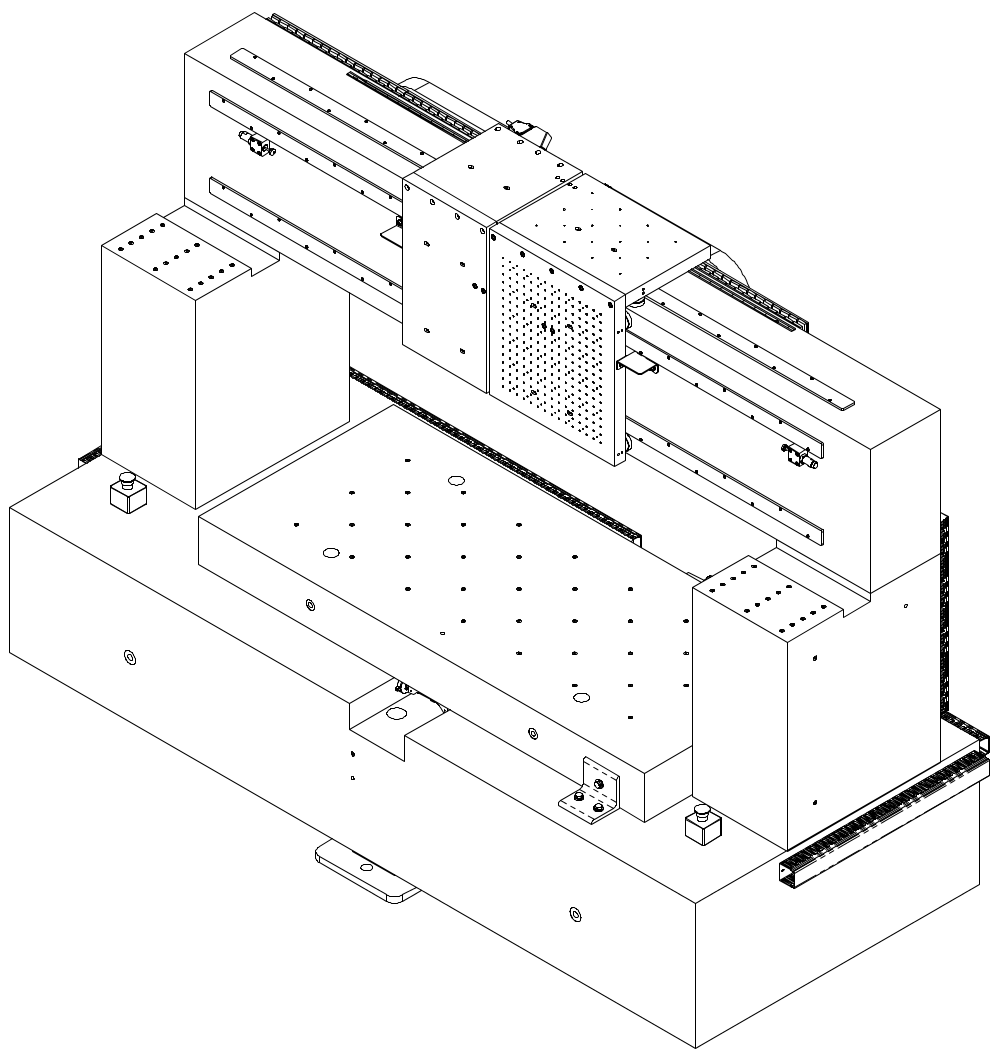
\includegraphics[width=\textwidth]{imgs/alba/laop/laop_ltp_isometric_view.png}
            \end{figure}
        \end{block}
    \end{textblock*}
    \begin{textblock*}{50mm}(0.65\textwidth,0.2\textheight)
        \begin{block}{From the clean room}<2->
            \begin{figure}
                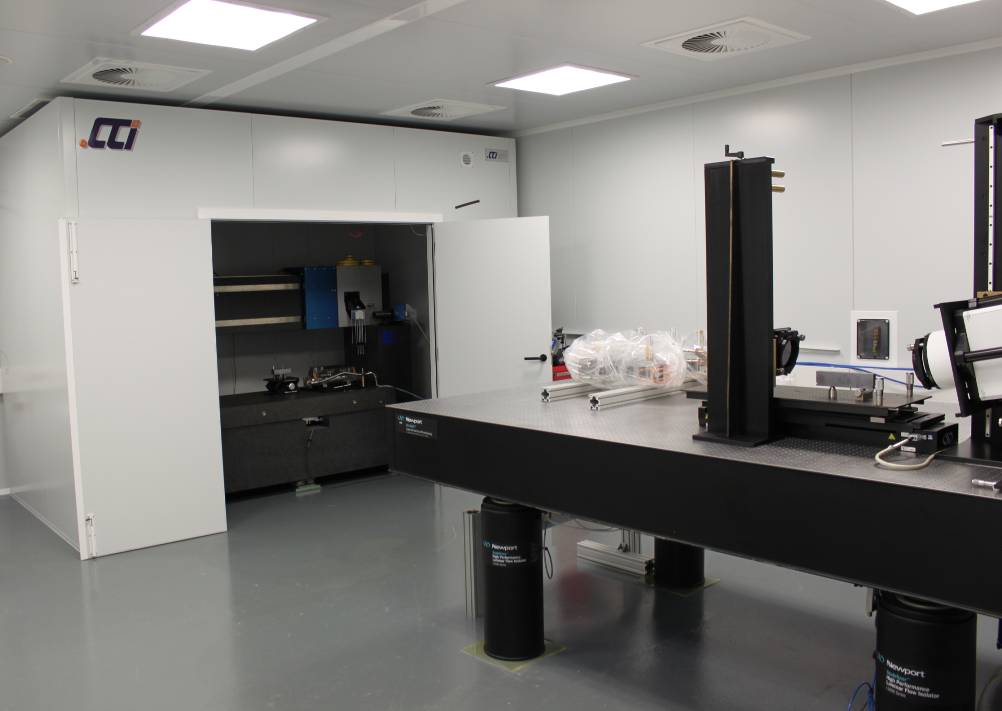
\includegraphics[width=\textwidth]{imgs/alba/laop/01_LTP_a_sala_blanca.jpg}
            \end{figure}
        \end{block}
    \end{textblock*}
    \begin{textblock*}{45mm}(0.675\textwidth,0.5\textheight)
        \begin{block}{Ambient temperature}<3->
            \begin{figure}
                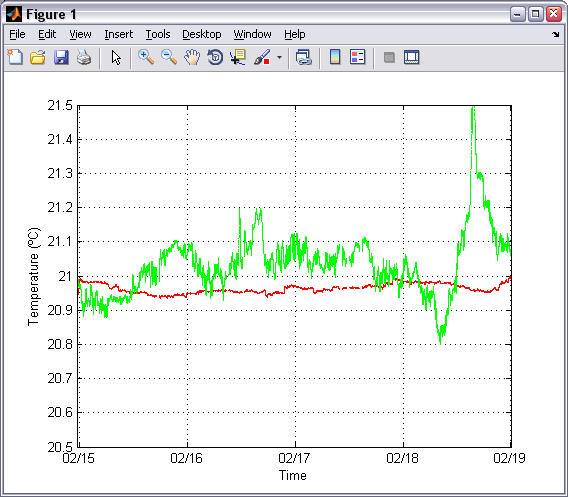
\includegraphics[width=\textwidth]{imgs/alba/laop/02_laop-temperatures.png}
            \end{figure}
        \end{block}
    \end{textblock*}
    \begin{textblock*}{45mm}(0.55\textwidth,0.2\textheight)
        \begin{exampleblock}{Mirror position}<4->
            \begin{figure}
                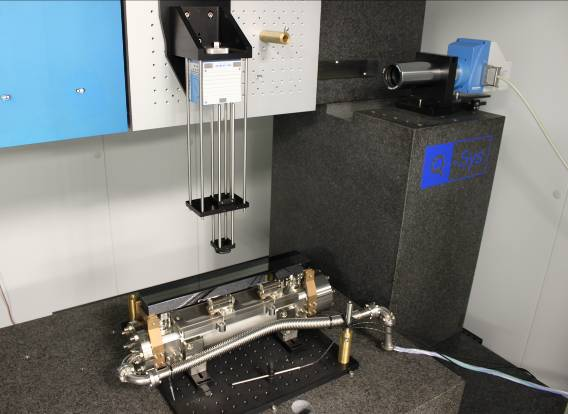
\includegraphics[width=\textwidth]{imgs/alba/laop/03_detall_LTP_normal_configuration.jpg}
            \end{figure}
        \end{exampleblock}
    \end{textblock*}
    \begin{textblock*}{45mm}(0.55\textwidth,0.6\textheight)
        \begin{exampleblock}{Inverted configuration}<5->
            \begin{figure}
                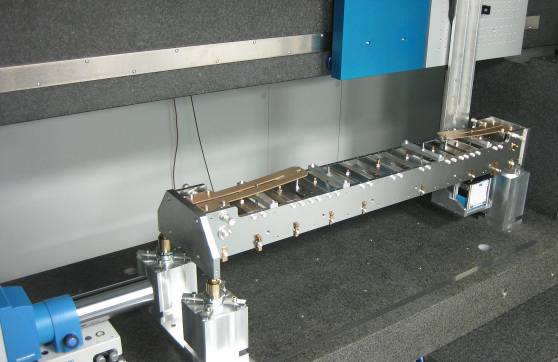
\includegraphics[width=\textwidth]{imgs/alba/laop/04_detall_LTP_inverted_configuration.jpg}
            \end{figure}
        \end{exampleblock}
    \end{textblock*}
    \begin{textblock*}{45mm}(0.075\textwidth,0.35\textheight)
        \begin{block}{Matlab GUI}<6->
            \begin{figure}
                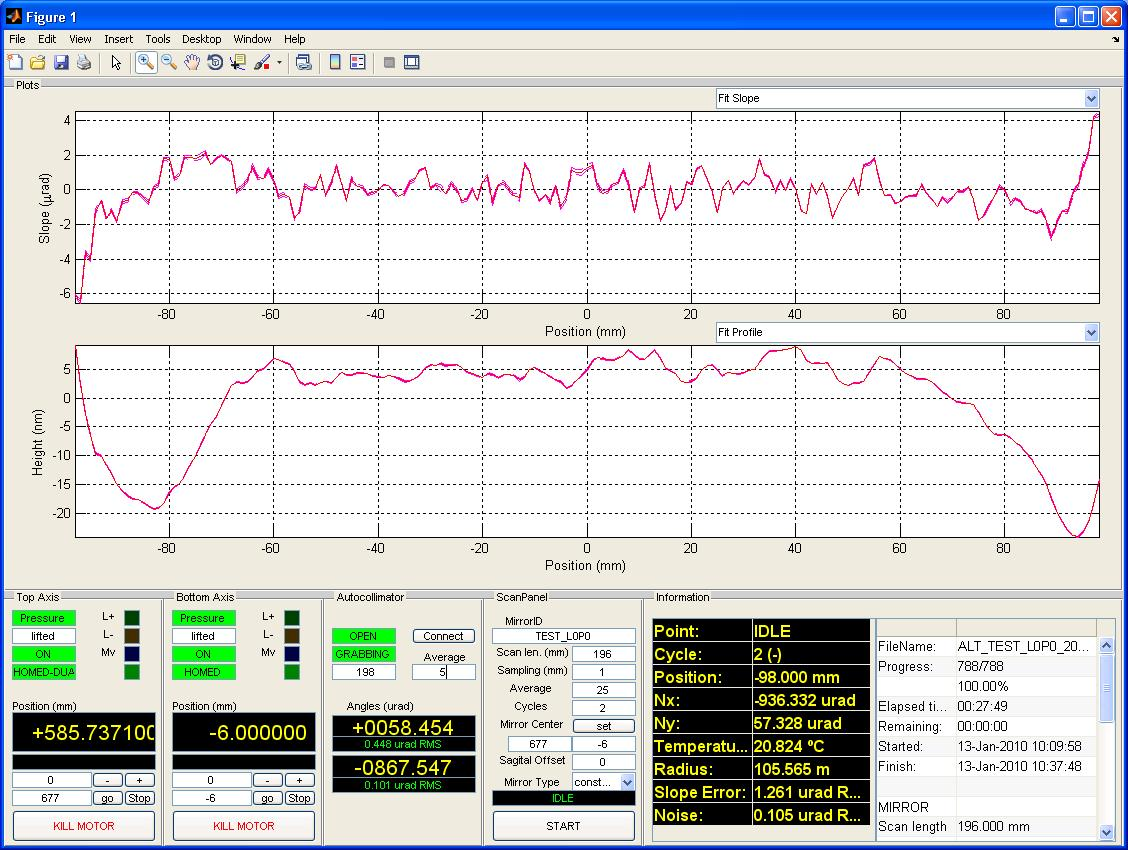
\includegraphics[width=\textwidth]{imgs/alba/laop/05_ltp_matlabgui.jpg}
            \end{figure}
        \end{block}
    \end{textblock*}
    \begin{textblock*}{45mm}(0.1\textwidth,0.7\textheight)
        \begin{exampleblock}{Surface example}<7->
            \begin{figure}
                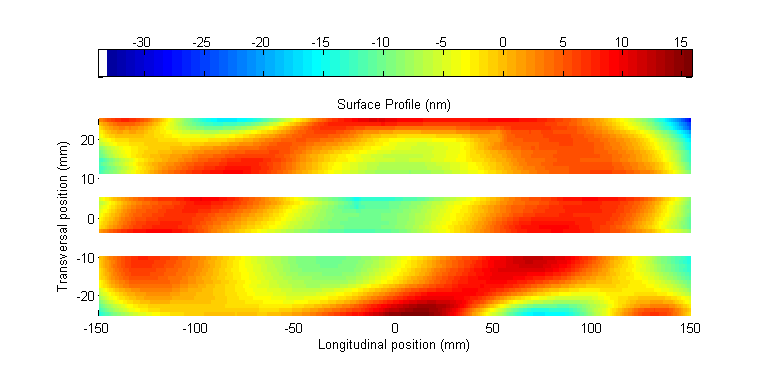
\includegraphics[width=\textwidth]{imgs/alba/laop/06_mirror_surface_example.png}
            \end{figure}
        \end{exampleblock}
    \end{textblock*}
    \begin{textblock*}{45mm}(0.6\textwidth,0.7\textheight)
        \begin{exampleblock}{Surface example}<8->
            \begin{figure}
                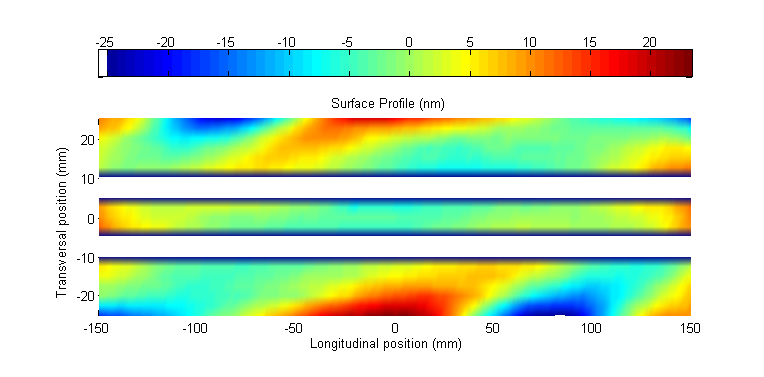
\includegraphics[width=\textwidth]{imgs/alba/laop/07_mirror_surface_example2.png}
            \end{figure}
        \end{exampleblock}
    \end{textblock*}
    \begin{textblock*}{35mm}(0.8\textwidth,0.25\textheight)
        \begin{exampleblock}{\tango information}<9->
            \begin{itemize}
                \item 3 Hosts
                \item 28 Devices
                \item 12 DServers
                \item 19 DClasses
            \end{itemize}
        \end{exampleblock}
    \end{textblock*}
    \begin{textblock*}{35mm}(0.8\textwidth,\textheight)
        \begin{block}{}
            \tiny{Images provided by Dr.Josep Nicolas}
        \end{block}
    \end{textblock*}
\end{frame}
%-----------------------------------------------------------------------------%

%------------------------------------ Frame 1.10 -----------------------------%
\begin{frame}
\frametitle{A beamline}
    \begin{textblock*}{100mm}(0.05\textwidth,0.2\textheight)
        \begin{block}{layout of BL11}
            \begin{figure}
                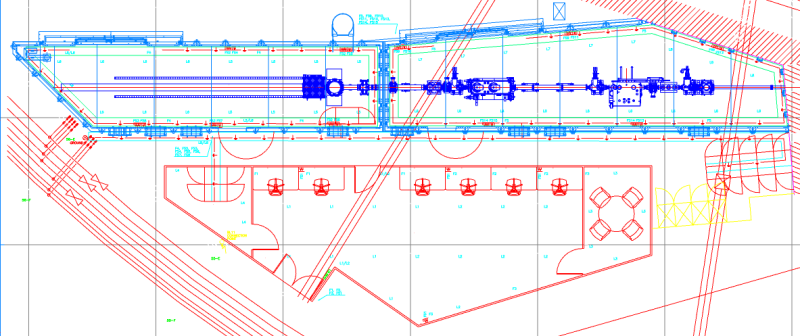
\includegraphics[width=\textwidth]{imgs/alba/2009_bl11_ncd.png}
            \end{figure}
        \end{block}
    \end{textblock*}
    \begin{textblock*}{100mm}(0.2\textwidth,0.3\textheight)
        \begin{block}{\sardana's gui in BL09}<2->
            \begin{figure}
                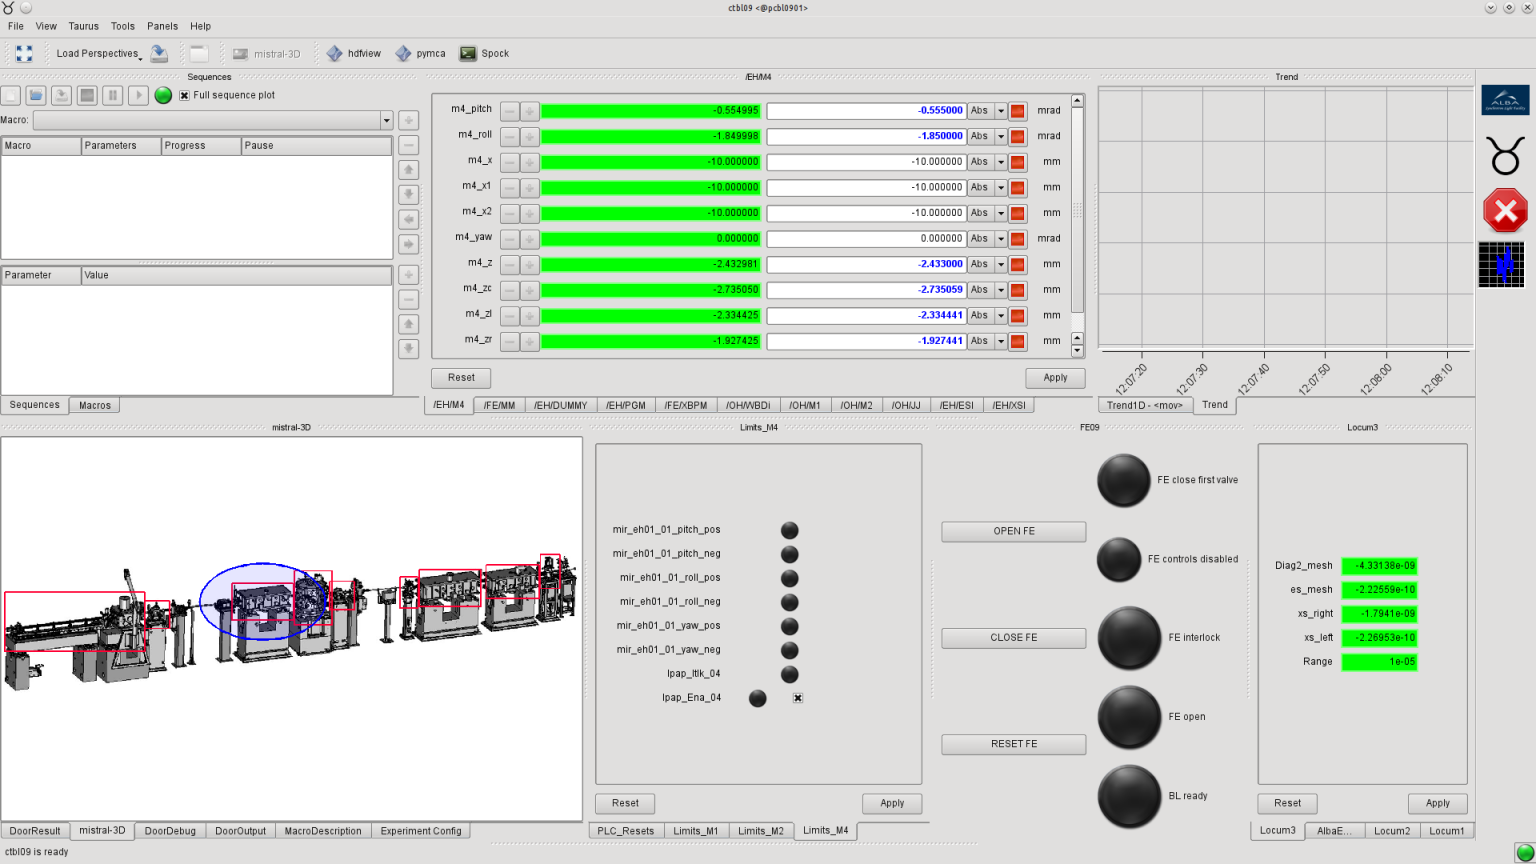
\includegraphics[width=\textwidth]{imgs/alba/20130917_ctbl09.png}
            \end{figure}
        \end{block}
    \end{textblock*}
    \begin{textblock*}{35mm}(0.8\textwidth,0.25\textheight)
        \begin{exampleblock}{\tango information (bl13)}<3->
            \begin{itemize}
                \item 7 Hosts
                \item 615 Devices
                \item 34 DServers
                \item 82 DClasses
            \end{itemize}
        \end{exampleblock}
    \end{textblock*}
\end{frame}
%-----------------------------------------------------------------------------%

%------------------------------------ Frame 1.11 -----------------------------%
\begin{frame}
\frametitle{Control a synchrotron accelerator}
    \begin{textblock*}{50mm}(0.05\textwidth,0.35\textheight)
        \begin{block}{Alba's overview}<1->
            \begin{figure}
                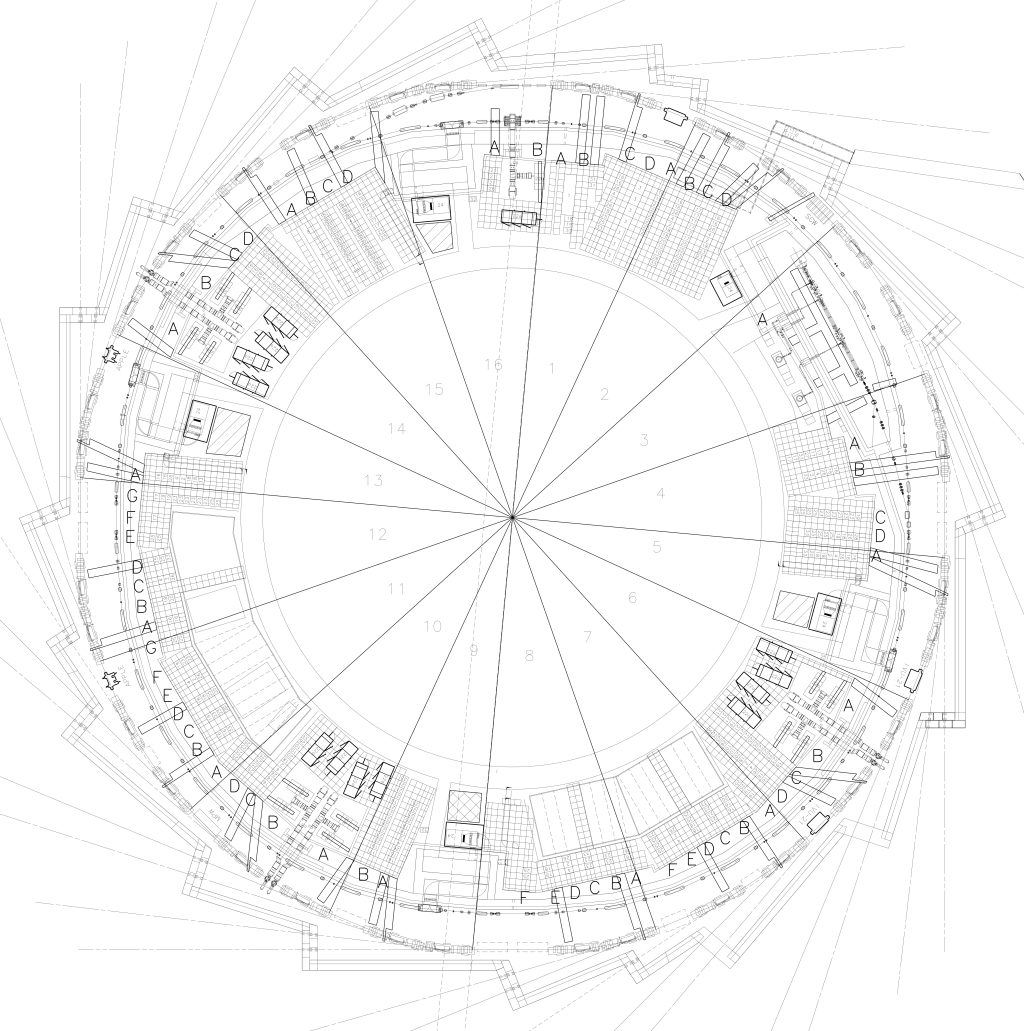
\includegraphics[width=\textwidth]{imgs/alba/Alba_overview.png}
            \end{figure}
        \end{block}
    \end{textblock*}
    \begin{textblock*}{50mm}(0.65\textwidth,0.45\textheight)
        \begin{block}{Alba's main network}<2->
            \begin{figure}
                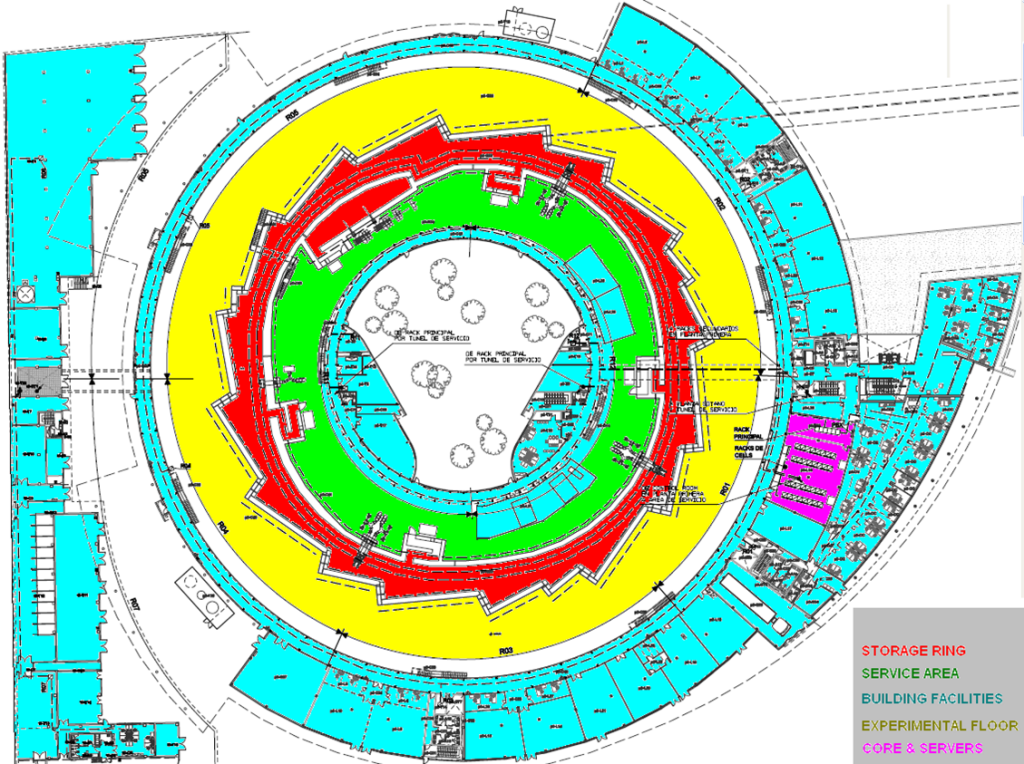
\includegraphics[width=\textwidth]{imgs/alba/Alba_MainNetwork.png}
            \end{figure}
        \end{block}
    \end{textblock*}
    \begin{textblock*}{50mm}(0.35\textwidth,0.2\textheight)
        \begin{block}{Alba's network layout}<3->
            \begin{figure}
                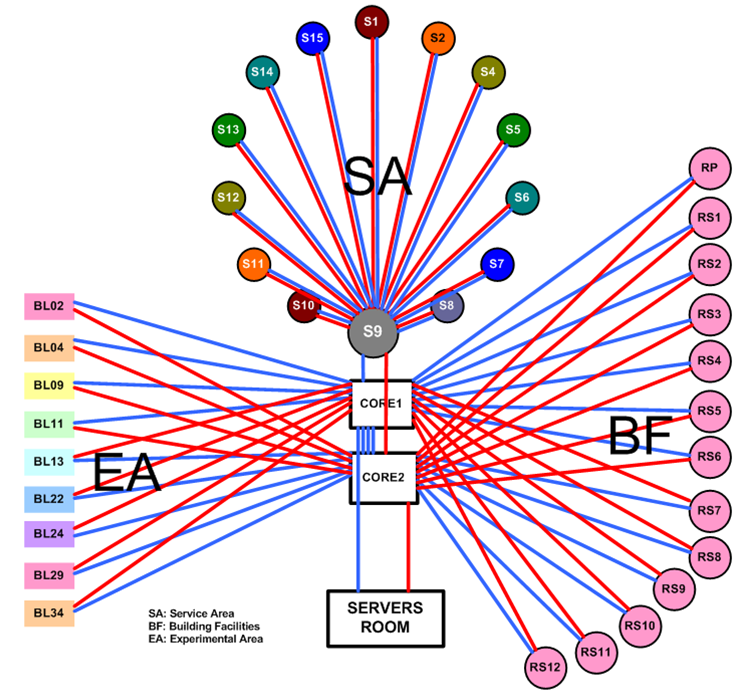
\includegraphics[width=\textwidth]{imgs/alba/Alba_NetworkLayout.png}
            \end{figure}
        \end{block}
    \end{textblock*}
    \begin{textblock*}{100mm}(0.15\textwidth,0.65\textheight)
        \begin{block}{Alba's Cabling Database}<4->
            \begin{figure}
                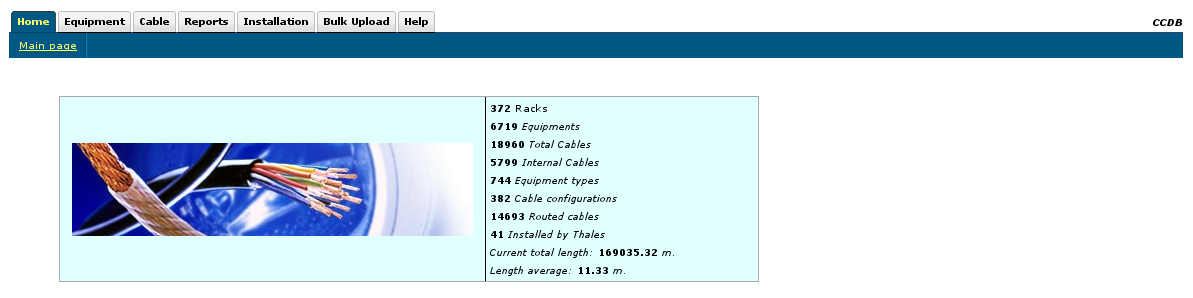
\includegraphics[width=\textwidth]{imgs/alba/20130916_ccdb.png}
            \end{figure}
        \end{block}
    \end{textblock*}
    \begin{textblock*}{35mm}(0.1\textwidth,0.25\textheight)
        \begin{block}{Alba's subsystems}<5->
            \begin{itemize}
                \item Timming %(132 agents)
                \item Vaccum %(1085 agents)
                \item Power supplies %(491 agents)
                \item Radio frequency %(124 agents)
                \item Diagnostics %(744 agents)
                \item EPS and PSS
                \item Fronted and IDs
            \end{itemize}
        \end{block}
    \end{textblock*}
    \begin{textblock*}{35mm}(0.8\textwidth,0.25\textheight)
        \begin{exampleblock}{\tango information (bl13)}<6->
            \begin{itemize}
                \item 139 Hosts
                \item 4259 Devices
                \item 85 DServers
                \item 1551 DClasses
            \end{itemize}
        \end{exampleblock}
    \end{textblock*}
\end{frame}
%-----------------------------------------------------------------------------%

%------------------------------------ Frame 1.12 -----------------------------%
\begin{frame}
\frametitle{Other possibilities}
    \begin{itemize}
        \item<2-> Factory production lines
        \item<3-> Critical factories
        \item<4-|alert@4-7> Electronic traffic lights and tools
        \item<8-|alert@8> Energy industry
    \end{itemize}
    %Production lines
    \begin{textblock*}{50mm}(0.6\textwidth,0.25\textheight)
        \begin{exampleblock}{Production lines}<2>
            \begin{figure}
                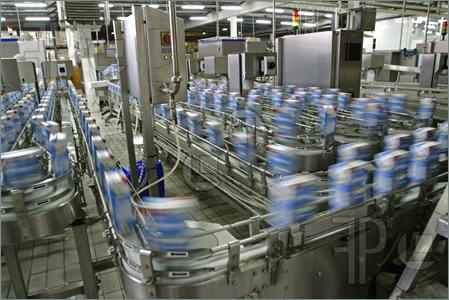
\includegraphics[width=\textwidth]{imgs/aux/Production-Line-Factory.jpg}
            \end{figure}
        \end{exampleblock}
    \end{textblock*}
    %More critical factories
    \begin{textblock*}{50mm}(0.6\textwidth,0.35\textheight)
        \begin{exampleblock}{Production lines}<3>
            \begin{figure}
                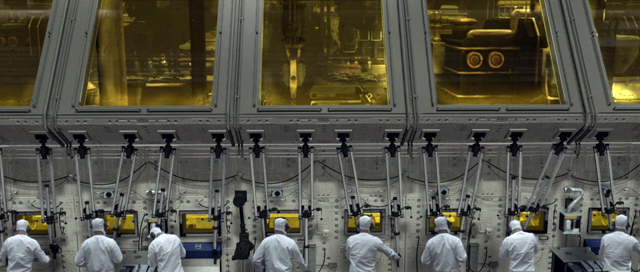
\includegraphics[width=\textwidth]{imgs/aux/THX_1138_DC.png}
            \end{figure}
        \end{exampleblock}
    \end{textblock*}
    %distributed exposed
    \begin{textblock*}{50mm}(0.6\textwidth,0.25\textheight)
        \begin{exampleblock}{Electronic road panels}<5-7>
            \begin{figure}
                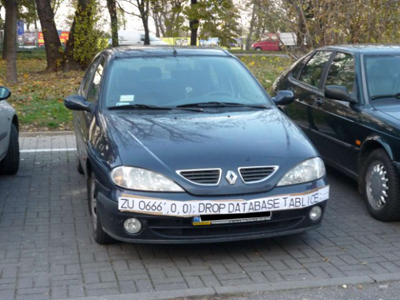
\includegraphics[width=\textwidth]{imgs/aux/plate_hack_sql.jpg}
            \end{figure}
        \end{exampleblock}
    \end{textblock*}
    \begin{textblock*}{50mm}(0.6\textwidth,0.35\textheight)
        \begin{exampleblock}{}<6-7>
            \begin{figure}
                
\includegraphics[width=\textwidth]{imgs/aux/youll_late_hack.jpg}
            \end{figure}
        \end{exampleblock}
    \end{textblock*}
    \begin{textblock*}{50mm}(0.6\textwidth,0.45\textheight)
        \begin{exampleblock}{}<7>
            \begin{figure}
                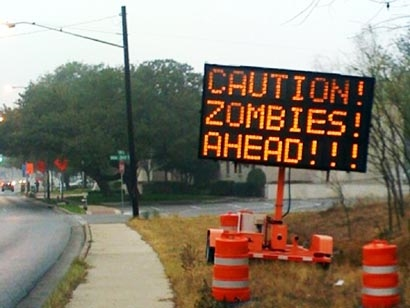
\includegraphics[width=\textwidth]{imgs/aux/zombies-ahead_hack.jpg}
            \end{figure}
        \end{exampleblock}
    \end{textblock*}
    \begin{textblock*}{42mm}(0.75\textwidth,\textheight)
        \begin{alertblock}{}
            \tiny{Images found in google, not license checked}
        \end{alertblock}
    \end{textblock*}
\end{frame}
%-----------------------------------------------------------------------------%

\subsection{In distributed system}

%------------------------------------ Frame 2.1 ------------------------------%
\begin{frame}
\frametitle{Against the transparencies}
    \resizebox{\textwidth}{!}{
        \begin{tabular}{|l|l|}
            \hline
            Access & Hide differences in data representation and how a resource is accessed \\ \hline
            Location & Hide where a resource is located \\ \hline
            Migration & Hide that a resource may move to another location \\ \hline
            Relocation & Hide that a resource may be moved to another location while in use \\ \hline
            Replication & Hide that a resource is replicated \\ \hline
            Concurrency & Hide that a resource may be shared by several competitive users \\ \hline
            Failure & Hide a faulure and recovery of a resource \\ \hline
            Persistence & Hide whether a (software) resource is in memory or on disk \\ \hline
        \end{tabular}
    }
    \begin{block}{Security threads}<2->
        All those transparencies shows at least on security issue
    \end{block}

\end{frame}
%-----------------------------------------------------------------------------%

% %------------------------------------ Frame 2.2 ------------------------------%
% \begin{frame}
% \frametitle{Against the layers}
%     \begin{figure}[h]
%         \centering{
%         %\resizebox{0.5\textwidth}{!}{% PSTricks TeX macro
% Title: /home/serguei/src/Papers/Ensuring_Tango_CtrlSys/imgs/TanenbaumDistributedSystemOrganization.dia
% Creator: Dia v0.97.2
% CreationDate: Sun Aug 11 19:16:03 2013
% For: serguei
% \usepackage{pstricks}
% The following commands are not supported in PSTricks at present
% We define them conditionally, so when they are implemented,
% this pstricks file will use them.
\ifx\setlinejoinmode\undefined
  \newcommand{\setlinejoinmode}[1]{}
\fi
\ifx\setlinecaps\undefined
  \newcommand{\setlinecaps}[1]{}
\fi
% This way define your own fonts mapping (for example with ifthen)
\ifx\setfont\undefined
  \newcommand{\setfont}[2]{}
\fi
\pspicture(3.900000,-19.100000)(24.100000,-5.386312)
\psscalebox{1.000000 -1.000000}{
\newrgbcolor{dialinecolor}{0.000000 0.000000 0.000000}%
\psset{linecolor=dialinecolor}
\newrgbcolor{diafillcolor}{1.000000 1.000000 1.000000}%
\psset{fillcolor=diafillcolor}
\psset{linewidth=0.100000cm}
\psset{linestyle=solid}
\psset{linestyle=solid}
\setlinejoinmode{0}
\newrgbcolor{dialinecolor}{0.000000 0.000000 0.000000}%
\psset{linecolor=dialinecolor}
\pspolygon(4.000000,7.000000)(4.000000,17.000000)(9.690000,17.000000)(9.690000,7.000000)
\psset{linewidth=0.100000cm}
\psset{linestyle=solid}
\psset{linestyle=solid}
\setlinejoinmode{0}
\newrgbcolor{dialinecolor}{0.000000 0.000000 0.000000}%
\psset{linecolor=dialinecolor}
\pspolygon(11.000000,7.000000)(11.000000,17.000000)(16.690000,17.000000)(16.690000,7.000000)
\psset{linewidth=0.100000cm}
\psset{linestyle=solid}
\psset{linestyle=solid}
\setlinejoinmode{0}
\newrgbcolor{dialinecolor}{0.000000 0.000000 0.000000}%
\psset{linecolor=dialinecolor}
\pspolygon(18.000000,7.000000)(18.000000,17.000000)(23.690000,17.000000)(23.690000,7.000000)
\psset{linewidth=0.100000cm}
\psset{linestyle=solid}
\psset{linestyle=solid}
\setlinejoinmode{0}
\newrgbcolor{dialinecolor}{1.000000 1.000000 1.000000}%
\psset{linecolor=dialinecolor}
\pspolygon*(5.000000,11.000000)(5.000000,13.000000)(23.000000,13.000000)(23.000000,11.000000)
\newrgbcolor{dialinecolor}{0.000000 0.000000 0.000000}%
\psset{linecolor=dialinecolor}
\pspolygon(5.000000,11.000000)(5.000000,13.000000)(23.000000,13.000000)(23.000000,11.000000)
\setfont{Helvetica}{0.800000}
\newrgbcolor{dialinecolor}{0.000000 0.000000 0.000000}%
\psset{linecolor=dialinecolor}
\rput(14.000000,12.000000){\psscalebox{1 -1}{Tango Middleware}}
\psset{linewidth=0.100000cm}
\psset{linestyle=solid}
\psset{linestyle=solid}
\setlinejoinmode{0}
\newrgbcolor{dialinecolor}{1.000000 1.000000 1.000000}%
\psset{linecolor=dialinecolor}
\pspolygon*(5.000000,8.000000)(5.000000,10.000000)(23.000000,10.000000)(23.000000,8.000000)
\newrgbcolor{dialinecolor}{0.000000 0.000000 0.000000}%
\psset{linecolor=dialinecolor}
\pspolygon(5.000000,8.000000)(5.000000,10.000000)(23.000000,10.000000)(23.000000,8.000000)
\setfont{Helvetica}{0.800000}
\newrgbcolor{dialinecolor}{0.000000 0.000000 0.000000}%
\psset{linecolor=dialinecolor}
\rput(14.000000,9.000000){\psscalebox{1 -1}{Distributed application}}
\psset{linewidth=0.100000cm}
\psset{linestyle=solid}
\psset{linestyle=solid}
\setlinejoinmode{0}
\newrgbcolor{dialinecolor}{0.000000 0.000000 0.000000}%
\psset{linecolor=dialinecolor}
\pspolygon(5.000000,14.000000)(5.000000,16.000000)(9.000000,16.000000)(9.000000,14.000000)
\setfont{Helvetica}{0.800000}
\newrgbcolor{dialinecolor}{0.000000 0.000000 0.000000}%
\psset{linecolor=dialinecolor}
\rput(7.000000,15.000000){\psscalebox{1 -1}{Local OS}}
\psset{linewidth=0.100000cm}
\psset{linestyle=solid}
\psset{linestyle=solid}
\setlinejoinmode{0}
\newrgbcolor{dialinecolor}{0.000000 0.000000 0.000000}%
\psset{linecolor=dialinecolor}
\pspolygon(12.000000,14.000000)(12.000000,16.000000)(16.000000,16.000000)(16.000000,14.000000)
\setfont{Helvetica}{0.800000}
\newrgbcolor{dialinecolor}{0.000000 0.000000 0.000000}%
\psset{linecolor=dialinecolor}
\rput(14.000000,15.000000){\psscalebox{1 -1}{Local OS}}
\psset{linewidth=0.100000cm}
\psset{linestyle=solid}
\psset{linestyle=solid}
\setlinejoinmode{0}
\newrgbcolor{dialinecolor}{0.000000 0.000000 0.000000}%
\psset{linecolor=dialinecolor}
\pspolygon(19.000000,14.000000)(19.000000,16.000000)(23.000000,16.000000)(23.000000,14.000000)
\setfont{Helvetica}{0.800000}
\newrgbcolor{dialinecolor}{0.000000 0.000000 0.000000}%
\psset{linecolor=dialinecolor}
\rput(21.000000,15.000000){\psscalebox{1 -1}{Local OS}}
\psset{linewidth=0.200000cm}
\psset{linestyle=solid}
\psset{linestyle=solid}
\setlinecaps{0}
\newrgbcolor{dialinecolor}{0.000000 0.000000 0.000000}%
\psset{linecolor=dialinecolor}
\psline(4.000000,19.000000)(24.000000,19.000000)
\psset{linewidth=0.200000cm}
\psset{linestyle=solid}
\psset{linestyle=solid}
\setlinecaps{0}
\newrgbcolor{dialinecolor}{0.000000 0.000000 0.000000}%
\psset{linecolor=dialinecolor}
\psline(7.000000,17.000000)(7.000000,19.000000)
\psset{linewidth=0.200000cm}
\psset{linestyle=solid}
\psset{linestyle=solid}
\setlinecaps{0}
\newrgbcolor{dialinecolor}{0.000000 0.000000 0.000000}%
\psset{linecolor=dialinecolor}
\psline(14.000000,17.000000)(14.000000,19.000000)
\psset{linewidth=0.200000cm}
\psset{linestyle=solid}
\psset{linestyle=solid}
\setlinecaps{0}
\newrgbcolor{dialinecolor}{0.000000 0.000000 0.000000}%
\psset{linecolor=dialinecolor}
\psline(21.000000,17.000000)(21.000000,19.000000)
\setfont{Helvetica}{0.800000}
\newrgbcolor{dialinecolor}{0.000000 0.000000 0.000000}%
\psset{linecolor=dialinecolor}
\rput[l](5.000000,4.000000){\psscalebox{1 -1}{}}
\setfont{Helvetica}{0.800000}
\newrgbcolor{dialinecolor}{0.000000 0.000000 0.000000}%
\psset{linecolor=dialinecolor}
\rput(7.000000,6.000000){\psscalebox{1 -1}{Machine A}}
\setfont{Helvetica}{0.800000}
\newrgbcolor{dialinecolor}{0.000000 0.000000 0.000000}%
\psset{linecolor=dialinecolor}
\rput(7.000000,6.800000){\psscalebox{1 -1}{}}
\setfont{Helvetica}{0.800000}
\newrgbcolor{dialinecolor}{0.000000 0.000000 0.000000}%
\psset{linecolor=dialinecolor}
\rput(14.000000,6.000000){\psscalebox{1 -1}{Machine B}}
\setfont{Helvetica}{0.800000}
\newrgbcolor{dialinecolor}{0.000000 0.000000 0.000000}%
\psset{linecolor=dialinecolor}
\rput(21.000000,6.000000){\psscalebox{1 -1}{Machine C}
\endpspicture}
%         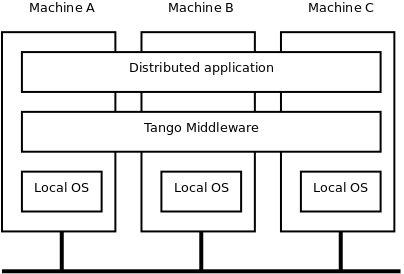
\includegraphics[width=0.5\textwidth]{imgs/TanenbaumDistributedSystemOrganization.png}
%         \caption{From \cite{TanenbaumDistr}, A distributed system organized as middleware} \label{fig:TanenbaumDistributedSystemOrganization}}
%     \end{figure}
% \end{frame}
% %-----------------------------------------------------------------------------%

\subsection{In security engineering}

%------------------------------------ Frame 2.3 ------------------------------%
\begin{frame}
\frametitle{Basics on \emph{information security}}
    \begin{enumerate}
        \item Confidentiality
        \uncover<2->{
            \begin{itemize}
                \item Information must be disclosed only to the authorized.
            \end{itemize}
        }
        \item Integrity
        \uncover<3->{
            \begin{itemize}
                \item Only authorized can set in the system.
            \end{itemize}
        }
        \item Availability
        \uncover<4->{
            \begin{itemize}
                \item Information must be accessible for those who are authorized.
            \end{itemize}
        }
        \item Authenticity
        \uncover<5->{
            \begin{itemize}
                \item Information must only be emitted by the authorized.
            \end{itemize}
        }
        \item Non-repudiation
        \uncover<6->{
            \begin{itemize}
                \item Forbid validity changes on the information emitters.
            \end{itemize}
        }
        %until here they are the bases of information security
        \uncover<8->{
            \item Auditory
            \begin{itemize}
                \item trace who access where\\ (extremely useful for a security breach analysis).
            \end{itemize}
        }
    \end{enumerate}
    \begin{block}{}<7>
        Those first 5 are the basics of the \href{http://en.wikipedia.org/wiki/Information_security}{Information Security}
    \end{block}
\end{frame}

% %-----------------------------------------------------------------------------%

\subsection{Vulnerable attacks}

%------------------------------------ Frame 2.4 ------------------------------%
\begin{frame}
\frametitle{Attacks}
    \begin{block}{Passive}
        \begin{itemize}
            \item Eavesdropping
        \end{itemize}
    \end{block}
    \begin{block}{Active}<2->
        \begin{itemize}
            \item Men-in-the-middle
            \item Spoofing: mask and falsify data
            \item Noise-Interruption-poisoning: Block transmissions
            \begin{itemize}
                \item Includes [D]DoS
            \end{itemize}
            \item Modification/Fabrication: agent impersonate
        \end{itemize}
    \end{block}
    \begin{block}{Counter-measures}<3->
        \begin{itemize}
            \item Intrusion detection and recovery
        \end{itemize}
    \end{block}
\end{frame}
%-----------------------------------------------------------------------------%

%%%%%%%%%%%%%%%%%%%%%%%%%%%%%%%%%%%%%%%%%%%%%%%%%%%%%%%%%%%%%%%%%%%%%%%%%%%%%%%
\section{Cryptography engineering}

\subsection{Security threads}

%------------------------------------ Frame 3.1 ------------------------------%
\begin{frame}
\frametitle{Security threads, policies and mechanisms}
    \begin{block}{}
        \tango\, needs the `\alert{s}', like http\alert{s}, stmp\alert{s}, imap\alert{s}, telnet (\alert{ssh}),...
    \end{block}
    \begin{itemize}
        \item<2-> Thread model:\\From ``Security engineering''\cite{SecEngRossAnderson},\\based on where the thread usually comes from
         \uncover<3->{
            \begin{itemize}
                \item Hospital
                \item Bank
                \item Military base
            \end{itemize}
        }
        \item<4-> References also in ``Cryptography Engineering''\cite{cryptoEngineering}.
        \item<5-> `Practical paranoia' from ``Practical cryptography''\cite{PractCryptoSchneier}:
        \uncover<6->{
            \begin{itemize}
                \item Identify threads
                \item Evaluate attack capabilities
            \end{itemize}
        }
    \end{itemize}
    \begin{alertblock}{}<7->
        Do not left all your security in \href{http://en.wikipedia.org/wiki/ISO/IEC_27000-series}{ISO/IEC 27000-series}!
    \end{alertblock}
\end{frame}
%-----------------------------------------------------------------------------%

\subsection{Labelling}

%------------------------------------ Frame 3.2 ------------------------------%
\begin{frame}
\frametitle{Security levels}
    European commission \emph{fiche 17} \\``Exchange of EU classified information'' \cite{fiche17EU}
    \begin{itemize}
        \item Open or Unclassified
        \item Confidential
        \item Secret
        \item Top-Secret
    \end{itemize}
   \begin{exampleblock}{Sub-classifications}<2->
       Elements in a group can have internal subsets. Agents with ``Top-secret'' access only under one subsystem, but ``Confidential'' under another.
   \end{exampleblock}
\end{frame}
%-----------------------------------------------------------------------------%

%%%%%%%%%%%%%%%%%%%%%%%%%%%%%%%%%%%%%%%%%%%%%%%%%%%%%%%%%%%%%%%%%%%%%%%%%%%%%%%
\section{Proposed solutions}

% authentication of agents and users
% encryption of data transmitted:
% - solutions for synchronous/asynchronous
% - solutions for events
% secure the tango-db access: query and write

\subsection{Authentication}

%------------------------------------ Frame 4.1 ------------------------------%
\begin{frame}
\frametitle{Authentication (I)}
    \begin{block}{}
        \begin{itemize}
            \item Agent authentication
            \item User authentication (PAM in Unix)
        \end{itemize}
        In TLS what is authenticated is the server, almost never the client.
    \end{block}
    \begin{block}{Rights}<2->
         Who have rights to do any read/write action\\
         \emph{Access Control Levels: would be similar than linux permissions}\\
         But multilevel and both directions.
    \end{block}
    \begin{alertblock}{Tools}<3->
        \begin{itemize}
            \item Elliptic curve cryptosystem for TLS (RFC4492 \cite{rfc4492})
            \item This one allow any curve (prime\&char2) in WRF\footnote{Weierstrass Reduced Form},\\unlike RFC6637 \cite{rfc6637}
        \end{itemize}
    \end{alertblock}
\end{frame}
%-----------------------------------------------------------------------------%

\subsection{Encryption}

%------------------------------------ Frame 4.2 ------------------------------%
\begin{frame}
\frametitle{Encryption}
    \begin{itemize}
        \item Encrypt \emph{what has send} to an agent and its \emph{answer}
        \item Encrypt \emph{events} emitted
    \end{itemize}
    \begin{exampleblock}{}<2->
        \begin{itemize}
            \item Transmissions from \emph{single booleans} to \emph{arrays of tenths of thousands of 64bit} elements.
            \item Neither forget the frequency that they can be transmitted.
        \end{itemize}
    \end{exampleblock}
    \begin{alertblock}{Tools}<3->
        \begin{itemize}
            \item Elliptic curves cryptosystem for \emph{key exchange}
            \item<4-> (generalized) Rijndael (data transmission \& event broadcasting)
            \begin{itemize}
                \item<5-> Smaller block size requested
                \item<5-> Bigger block size would be better than block cipher modes (CBC, CFB, CTR)
            \end{itemize}
            \item<6-> Stream ciphers
        \end{itemize}
    \end{alertblock}
\end{frame}
%-----------------------------------------------------------------------------%

%------------------------------------ Frame 4.3 ------------------------------%
\begin{frame}
\frametitle{ECC authentication \& encryption}
    \begin{block}{Using different curves}<2->
        \begin{itemize}
            \item<2-> Each security level requires its curve size (\Fp)
            \item<3-> Different \emph{subsystems} must use different curves.\\(even if they have same level)
        \end{itemize}
    \end{block}
    \begin{textblock*}{40mm}(0.75\textwidth,0.225\textheight)
        \begin{exampleblock}{Certicom's curves \cite{sec2}}<4->
            They are not enough.\\\small{(Superset NIST curves).}
        \end{exampleblock}
    \end{textblock*}
    \begin{alertblock}{Tools}<5->
        Auditable EC generation algorithm.
    \end{alertblock}
    \begin{textblock*}{45mm}(0.7\textwidth,0.525\textheight)
        \begin{exampleblock}{Cryptosetup}<6->
            Institution (re)set
        \end{exampleblock}
    \end{textblock*}
    \begin{exampleblock}{Collateral help}<7->
        This would help to avoid to share same curve between too many.\\Thread that the X9.62 \cite{X9.62-1998} advice.
    \end{exampleblock}
\end{frame}
%-----------------------------------------------------------------------------%

\subsection{Database}

%------------------------------------ Frame 4.4 ------------------------------%
\begin{frame}
\frametitle{Database access}
    \begin{itemize}
        \item \tango-db is the ``phone guide'' of the system\\also stores persistent data, like the properties
        \item<2-> It is necessary to record over the properties:
        \begin{itemize}
            \item<2-> Who and when modifies
            \item<2-> Who and when reads (read should be also protectable)
        \end{itemize}
        \item<3-> Should be possible to restrict areas of the ``phone book''
        \begin{itemize}
            \item<3-> It doesn't have much sense to say where an agent runs if you don't have right to talk with it
            \item<3-> this must not replace agent request for authentication of the requester.
        \end{itemize}
    \end{itemize}
    \begin{alertblock}{Tools}<4->
        \begin{itemize}
            \item Homomorphic encryption/Ordered cryptography
        \end{itemize}
    \end{alertblock}
\end{frame}
%-----------------------------------------------------------------------------%

%%%%%%%%%%%%%%%%%%%%%%%%%%%%%%%%%%%%%%%%%%%%%%%%%%%%%%%%%%%%%%%%%%%%%%%%%%%%%%%
\section{Reference Papers}

\frame{\tableofcontents[sectionstyle=show/hide,subsectionstyle=show/show/hide]}

%------------------------------------ Frame 5.1 ------------------------------%
\begin{frame}
\frametitle{(free) Paper sources}
\begin{itemize}
 \item \href{http://www.iacr.org/}{International Association for Cryptologic Research}\\(e-print \& archiver)
 \item \href{http://arxiv.org(}{arxiv} (open access e-print archiver)
 \item \href{http://vixra.org/}{vixra} (alternative open e-print archiver)
 \item \href{http://citeseerx.ist.psu.edu/}{citeseer} (scientific search engine)
 \item \href{http://scholar.google.com/}{scholar} (Google's indexer)
 \item \href{http://www.informatik.uni-trier.de/~ley/db/}{dblp} (bib reference)
\end{itemize} 
\end{frame}
%-----------------------------------------------------------------------------%

\subsection{Zero-knowledge proof}

%------------------------------------ Frame 5.2 ------------------------------%
\begin{frame}
\frametitle{Zero-knowledge proof for authentication}
    \begin{itemize}
        \item S.Mart\'{\i}nez, ``\emph{Protocolos de seguridad para sistemas de identificaci\'on por radiofrecuencia}''. PhD Thesis UdL, march 2011. Directed by: Concepci\'o Roig and Magda Valls.\cite{Santi11}
        \item BSI TR-03110:``\emph{Advanced security mechanisms for machine readable travel documents.}''.\cite{BSI_TR-03110}
    \end{itemize}
\end{frame}
%-----------------------------------------------------------------------------%

\subsection{Session key exchange}

%------------------------------------ Frame 5.3 ------------------------------%
\begin{frame}
\frametitle{key exchange}
    \begin{itemize}
        \item R. Tom\`as, ``\emph{Volcans d'isogenies de corbes el$\cdot$l\'{\i}ptiques: Aplicacions criptogr\`afiques en targetes intel$\cdot$ligents}''. PhD Thesis UdL, march 2011. Directed by: Josep M. Miret and Daniel Sadornil.\cite{Rosana11}
        \item BSI TR-03111:``\emph{Elliptic curve cryptography, version 2.0}''.\cite{BSI_TR-03111}
        \item S. Blake-Wilson, N. Bolyard, V. Gupta, C. Hawk, and B. Moeller, ``\emph{Elliptic curve cryptography (ecc) cipher suites for transport layer security (tls)}'' May 2006. RFC4492. \cite{rfc4492}
    \end{itemize}
\end{frame}
%-----------------------------------------------------------------------------%

%------------------------------------ Frame 5.3 ------------------------------%
\begin{frame}
\frametitle{Elliptic curves}
    \begin{itemize}
        \item J. Valera, “Volcales de $\ell$-isogenias de curvas elípticas,” Sistemas Informáticos. Escola Politècnica Superior. Universidad de Lleida, Sept 2011. Directed by: Josep M. Miret. \cite{JValera11}
        \item A. Rostovtsev and E. Rostovtsev and A. Stolbunov ``Public-Key Cryptosystem Based On''. 2006 \cite{Rostovtsev06public}
        \item R. Moreno, Subgrupos de Sylow de las curva ellíıpticas definidas sobre cuerpos finitos. PhD thesis, Universitat Politècnica de Catalunya, 2005. Directed by: Anna Rio and Josep M. Miret. \cite{ramiro05}
    \end{itemize}
    Ongoing:
    \begin{itemize}
        \item S. Blanch-Torn\'e and R. Moreno and F. Seb\'e and J. Varela ``Security risk associated with multiple users sharing the same elliptic curve''. Draft \cite{secRickShareECs}
    \end{itemize}

\end{frame}
%-----------------------------------------------------------------------------%

% \subsection{Secret broadcasting}
% 
% %------------------------------------ Frame 5.4 ------------------------------%
% \begin{frame}
% \frametitle{Secret broadcasting}
% \end{frame}
% %-----------------------------------------------------------------------------%

\subsection{Symmetric and stream ciphers}

%------------------------------------ Frame 5.5 ------------------------------%
\begin{frame}
\frametitle{Symmetric ciphers}
    \begin{itemize}
        \item ``\emph{Specification for the advanced encryption standard (aes).}'' Federal Information Processing Standards Publication 197, 2001.\cite{AES-FIPS}
        \item J. Daemen and V. Rijmen, ``\emph{The Design of Rijndael}''. Secaucus, NJ, USA: Springer-Verlag New York, Inc., 2002. \cite{Daemen:2002:DR:560131}
        \item J. Schaad and R. Housley, ``\emph{Advanced Encryption Standard (AES) Key Wrap Algorithm.}'' Sept. 2002. RFC3394 \cite{rfc3394}
    \end{itemize}
    Ongoing:
    \begin{itemize}
        \item S. Blanch-Torn\'e and R. Moreno and F. Seb\'e and M. Valls ``Generalised Rijndael''. Draft \cite{gRijndael}
    \end{itemize}
\end{frame}
%-----------------------------------------------------------------------------%

%------------------------------------ Frame 5.6 ------------------------------%
\begin{frame}
\frametitle{Stream ciphers}
    \begin{itemize}
        \item \todo{More information required!}
        \item Key Derivation Functions
        \item \href{http://en.wikipedia.org/wiki/Stream_cipher\#Comparison_Of_Stream_Ciphers}{Wikipedia (en)}
        \begin{itemize}
            \item \href{http://en.wikipedia.org/wiki/Rabbit_(cipher)}{Rabbit} (\href{http://tools.ietf.org/html/rfc4503}{RFC4503})
            \item \href{http://en.wikipedia.org/wiki/VEST}{VEST}
        \end{itemize}
        \item \href{http://godoc.org/github.com/codahale/chacha20}{Chacha20}
     \end{itemize}
\end{frame}
%-----------------------------------------------------------------------------%

\subsection{Homomorphic encryption}

%------------------------------------ Frame 5.7 ------------------------------%
\begin{frame}
\frametitle{Private database query system}
    \begin{itemize}
        \item D. B. nad Craig Bentry, S. Halevi, F. Wang, and D. J. Wu, ``\emph{Private database queries using somewhat homomorphic encryption,}'' International Association for Cryptologic Research, June 2013.
    \end{itemize}
\end{frame}
%-----------------------------------------------------------------------------%

%%%%%%%%%%%%%%%%%%%%%%%%%%%%%%%%%%%%%%%%%%%%%%%%%%%%%%%%%%%%%%%%%%%%%%%%%%%%%%%
\section{Journals \& Conferences}

\subsection{Journals}

%------------------------------------ Frame 6.1 ------------------------------%
\begin{frame}
\frametitle{Reference journals}
    \begin{itemize}
        \item \todo{More information required!}
    \end{itemize}
\end{frame}
%-----------------------------------------------------------------------------%

\subsection{Conferences}

%------------------------------------ Frame 6.2 ------------------------------%
\begin{frame}
\frametitle{Reference conferences \& workshops}
\begin{itemize}
    \item \href{http://www.icalepcs.org/}{Icalepcs}: International Conference on Accelerator and Large Experimental Physics Control Systems
    \item \href{http://www.nobugsconference.org/}{No-bugs}: New Opportunities for Better User Group Software
    \item \href{http://www.chesworkshop.org/}{CHES}: Cryptographic Hardware and Embedded Systems
    \item \href{http://www.sacconference.org/}{SAC}: Selected Areas in Cryptography
          % Montreal, Canada
    \item Crypto, \href{http://www.iacr.org/meetings/eurocrypt/}{Eurocrypt}, \& Asiacrypt
          % Submission Deadline: Oct 17, 2013
          % dates for the conference: 11 – 15 May 2014 (Copenhagen, Denmark)
    \item Tango Meeting
\end{itemize}

\end{frame}
%-----------------------------------------------------------------------------%

%%%%%%%%%%%%%%%%%%%%%%%%%%%%%%%%%%%%%%%%%%%%%%%%%%%%%%%%%%%%%%%%%%%%%%%%%%%%%%%
\section*{Extra slides}

%------------------------------------ Frame 7.1 ------------------------------%
\begin{frame}[allowframebreaks]
        \frametitle{References}
        %\bibliographystyle{amsalpha}
        \bibliographystyle{ieeetr}
        \bibliography{../bibtex/books.bib,../bibtex/standards.bib,../bibtex/rfc.bib,../bibtex/ecc.bib,../bibtex/rijndael.bib,../bibtex/isogeny.bib,../bibtex/sblanch.bib}
\end{frame}
%-----------------------------------------------------------------------------%

%------------------------------------ Frame 7.2 ------------------------------%
\begin{frame}
\frametitle{Alba's \href{https://www.cells.es/Members/sblanch}{duties}}
    \begin{textblock*}{40mm}(0.0\textwidth,0.2\textheight)
        \begin{itemize}
            \item Diagnostics
            \begin{itemize}
                \item<alert@1> CCDs
                \item Instrumentation
                \item Tune excitation
                \item Filling Pattern FCT
            \end{itemize}
            \item<alert@1> Linac
            \item Power Supplies
            \begin{itemize}
                \item Magnet cycling
                \item StateCode interpreter
                \item<alert@1> Fast orbit feedback
            \end{itemize}
        \end{itemize}
    \end{textblock*}
    \begin{textblock*}{45mm}(0.325\textwidth,0.2\textheight)
        \begin{itemize}
            \item Radio Frequency
            \begin{itemize}
                \item Digital Low Level RF
                \item<alert@1> Fast Data Logger
                \item Facade
            \end{itemize}
            \item Optics lab
            \begin{itemize}
                \item Autocollimator
            \end{itemize}
            \item Sardana controllers
            \begin{itemize}
                \item IBACtrl
                \item ElComatCtrl
                \item AttenIOR (group)
                \item MirrorPM \& MonoPM
            \end{itemize}
        \end{itemize}
    \end{textblock*}
    \begin{textblock*}{55mm}(0.7\textwidth,0.2\textheight)
        \begin{itemize}
            \item Tango naming convention (and DNS)
            \item ``Interfaces to the Alba Control System''
            \item<alert@1> ``Controls coding standard and packaging convention''
        \end{itemize}
    \end{textblock*}
\end{frame}
%-----------------------------------------------------------------------------%

\end{document}


